% Une ligne commentaire débute par le caractère « % »

\documentclass[a4paper]{article}

% Options possibles : 10pt, 11pt, 12pt (taille de la fonte)
%                     oneside, twoside (recto simple, recto-verso)
%                     draft, final (stade de développement)

\usepackage[utf8]{inputenc}   % LaTeX, comprends les accents !
\usepackage[T1]{fontenc}      % Police contenant les caractères français
\usepackage[francais]{babel}  


\usepackage[a4paper,left=2cm,right=2cm]{geometry}% Format de la page, réduction des marges
\usepackage{graphicx}  % pour inclure des images

%\pagestyle{headings}        % Pour mettre des entêtes avec les titres
                              % des sections en haut de page

 \title{  Qui est-ce ?\\         % Les paramètres du titre : titre, auteur, date
  Projet de programmation}          
\author{Groupe \emph{Z}\\
  \emph{Frédéric,Laurent,Tony et Romain}\\
  \emph{git:git@gitlab.etu.umontpellier.fr:e20180001091/qui-est-ce.git}\\
  L2 informatique\\
  Faculté des Sciences\\
Université de Montpellier.}
\date{\today}             


\begin{document}

\maketitle                    % Faire un titre utilisant les données
                              % passées à \title, \author et \date

\begin{center}               % pour centrer 
  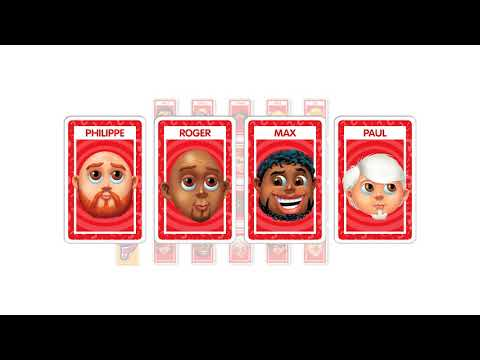
\includegraphics[scale=1]{img.jpg}   % insertion d'une image
\end{center}

\begin{abstract}     % Résumé du travail

  \emph{Description très succinte du problème et des différentes étapes de réalisation}

\end{abstract}



\section{Technologies utilisées  et organisation}



\subsection{Choix du langage}
\paragraph*{Nous avons choisi Python,} il s'agit d'un langage populaire avec une communauté active et nous n'avons pas eu de mal à trouver de l'aide ou des exemples.
De plus, le langage est simple et sa syntaxe courte nous a permis de réaliser notre projet relativement rapidement.
Puisque Python est Orienté Objet, nous avons réussi a mettre une structure du code acceptable.
La POO nous a permis de diviser les tâches à réaliser et les répartir facilement.
Finalement le code sera portable (Write Once, Run Anywhere) et cela nous a été précieux étant donnée que nous n'utilions pas le même environnement de travail.
\paragraph*{Bibliothèques, framework, ... utilisés:}
\begin{itemize}
\item Tkinter est installé par défaut sinon éxécuter (python3 -m tkinter) depuis la ligne de commande.Cela ouvrira une fenêtre de démonstration d'une interface Tk simple en indiquant que tkinter est correctement installé sur votre système et indiquant également quelle version de Tcl/Tk est installée\\
\end{itemize}

\subsection{Organisation du travail}
\paragraph{Répartition du travail au sein du groupe}

  - 4 personnes au sein du groupe: Romain, Frédéric ,Laurent et Tony
  \subparagraph{}
  Jeu de base:
  \begin{itemize}
  \item Romain : fonctions du jeu de base + interface graphique
  \item Frédéric : interface graphique
  \item Laurent + Tony : fonctions du jeu de base
  \end{itemize}

  \subparagraph{Générateur:}

  \begin{itemize}
    \item Frédéric : fonctions du générateur
    \item Tony : fonctions du générateur
    \item Laurent : Interface du générateur + fonctions du générateur 
    \item Romain : Interface du générateur
  \end{itemize}
   
   
\paragraph{Rythme de travail:} 3h/semaine en td + heures suplémentaires à la BU \\
 \subparagraph{Mode de fonctionnement:}
 \begin{itemize}
 \item Premier partie ->   modele UML + organisation des taches à se répartir\\
 \item Deuxième partie ->  Exécution de l'organisation  
 \end{itemize}

\end{document}

